\chapter{Bayesian Hyper-Heuristic}\label{chap:bhh}

\begin{quotation}
      ``The result is a posterior distribution, which the agent may use as its new prior in the next step.''
\end{quotation}
\begin{flushright}
      - Pedro Domingos, The Master Algorithm
\end{flushright}

The above quote was the inspiration for the development of a novel \acf{HH} that uses Bayesian probability concepts as a selection mechanism to drive the heuristic selection process. Thus far the reader has been presented with all of the necessary background information on \acp{ANN} (Chapter \ref{chap:anns}), low-level \index{heuristic}heuristics (Chapter \ref{chap:heuristics}), \acp{HH} (Chapter \ref{chap:hhs}) and lastly, probability theory (Chapter \ref{chap:probability}). These elements form the fundamental components of the proposed \Acf{BHH}. This chapter provides the details around the implementation of the \Ac{BHH} and explains how it is used to train \acp{FFNN}. The remainder of the chapter is structured as follows:

\begin{itemize}
      \item \textbf{Section \ref{sec:bhh:overview}} provides a brief overview of the \Acs{BHH}.

      \item \textbf{Section \ref{sec:bhh:architecture}} provides the general architecture and \Ac{HH} framework implemented by the \Acs{BHH}.

      \item \textbf{Section \ref{sec:bhh:heuristic_pool}} presents the \index{heuristic}\textit{heuristic pool}, a collection of low-level \index{heuristic}heuristics. Discussions follow on the importance of diversity amongst heuristics in the \index{heuristic pool}heuristic pool.

      \item \textbf{Section \ref{sec:bhh:entity_pool}} presents details on entity (local) and population (global) memory (state).

      \item \textbf{Section \ref{sec:bhh:performance_log}} presents detailed discussions on performance measurement. The \textit{performance log}, implemented by the \acs{BHH}, is presented.

      \item \textbf{Section \ref{sec:bhh:credit_assignment_strategy}} presents detailed discussions on credit assignment strategies.

      \item \textbf{Section \ref{sec:bhh:selection_mechanism}} presents the Bayesian probabilistic model that is used as the heuristic selection mechanism.

      \item \textbf{Section \ref{sec:bhh:optimisation_step}} presents the learning mechanisms by which the probabilistic model can be optimised.

      \item \textbf{Section \ref{sec:bhh:hyper_parameters}} summarises and discusses the associated \index{hyper-parameters}hyper-parameters and default values.

      \item \textbf{Section \ref{sec:bhh:algorithm}} provides the pseudo-code algorithm for the \acs{BHH}.

      \item \textbf{Section \ref{sec:bhh:summary}} provides a brief summary of the chapter.
\end{itemize}


\section{Overview}\label{sec:bhh:overview}

This section provides an overview of the workings of the \Acf{BHH}. The general concept of the \acs{BHH} can be summarised as follows: The \acs{BHH} implements a high-level heuristic selection mechanism that learns to select the best heuristic from a pool of low-level heuristics, to apply to a population of entities, each implementing a candidate solution to a \acs{FFNN}, with the intent of both optimising the underlying \acs{FFNN} and \acs{FFNN} training process. The \acs{BHH} does so by learning the probability that a given heuristic will perform well at a given stage in the \acs{FFNN} training process. These probabilities are then used as heuristic selection probabilities in the next step of the training process.

Formal classification of the \Acs{BHH} is needed. Chapter \ref{chap:hhs} presented the reader with a proposed classification scheme for \acp{HH} by~\citeauthor{ref:burke:2010}~\cite{ref:burke:2010}. According to the aforementioned classification scheme, the \Acs{BHH} is a population-based, meta-hyper-heuristic that utilises selection and perturbation of low-level heuristics in an online learning fashion. A breakdown of the classification is given as follows:

\begin{itemize}
      \item \textbf{Population-Based:} The \acs{BHH} implements a population-based approach, where a collection of different candidate solutions, referred to as \textit{entities}, work together to yield a global best solution.

      \item \textbf{Meta-Hyper-Heuristic:} There exists a domain barrier, where the \acs{BHH} searches through the \textit{heuristic space}, using only \index{heuristic}heuristic performance information, while lower level heuristics search through the \textit{solution space} using information from the search domain itself. Furthermore, the \index{heuristic pool}heuristic pool implemented by the \acs{BHH} supports both gradient-based low level \index{heuristic}heuristics, as well as meta-heuristics.

      \item \textbf{Selection and Perturbation of Low-Level Heuristics:} The \acs{BHH} implements a \index{heuristic}heuristic selection mechanism that selects from a collection of lower level \index{heuristic}heuristics, called a \index{heuristic pool}\textit{heuristic pool}. Selection is biased towards good performing heuristics. A credit assignment strategy is used to \textit{reward} good heuristic performance. The \acs{BHH} maintains entity and population state through operations that \textit{proxy} update steps from different heuristics (perturbation), as is required. These proxy operations ensure that heuristic requirements are satisfied even when different heuristics are used for different entities throughout the training process.

      \item \textbf{Online Learning:} The \acs{BHH} applies learning, at specified intervals, throughout the \acs{FFNN} training process.
\end{itemize}

\section{Architecture}\label{sec:bhh:architecture}

This section aims to present the reader with all the high level components in the architecture of the \Acs{BHH}. Burke et al.~\cite{ref:burke:2010} propose an initial framework for \acp{HH} and Grobler~\cite{ref:grobler:2015} further propose a framework for a heterogeneous meta-\ac{HH}. The aforementioned frameworks are adapted for the implementation of the \Acs{BHH}. An illustration of the high-level architecture of the \Acs{BHH} is given in Figure \ref{fig:bhh_architecture}.

\begin{figure}[htbp]
      \centering
      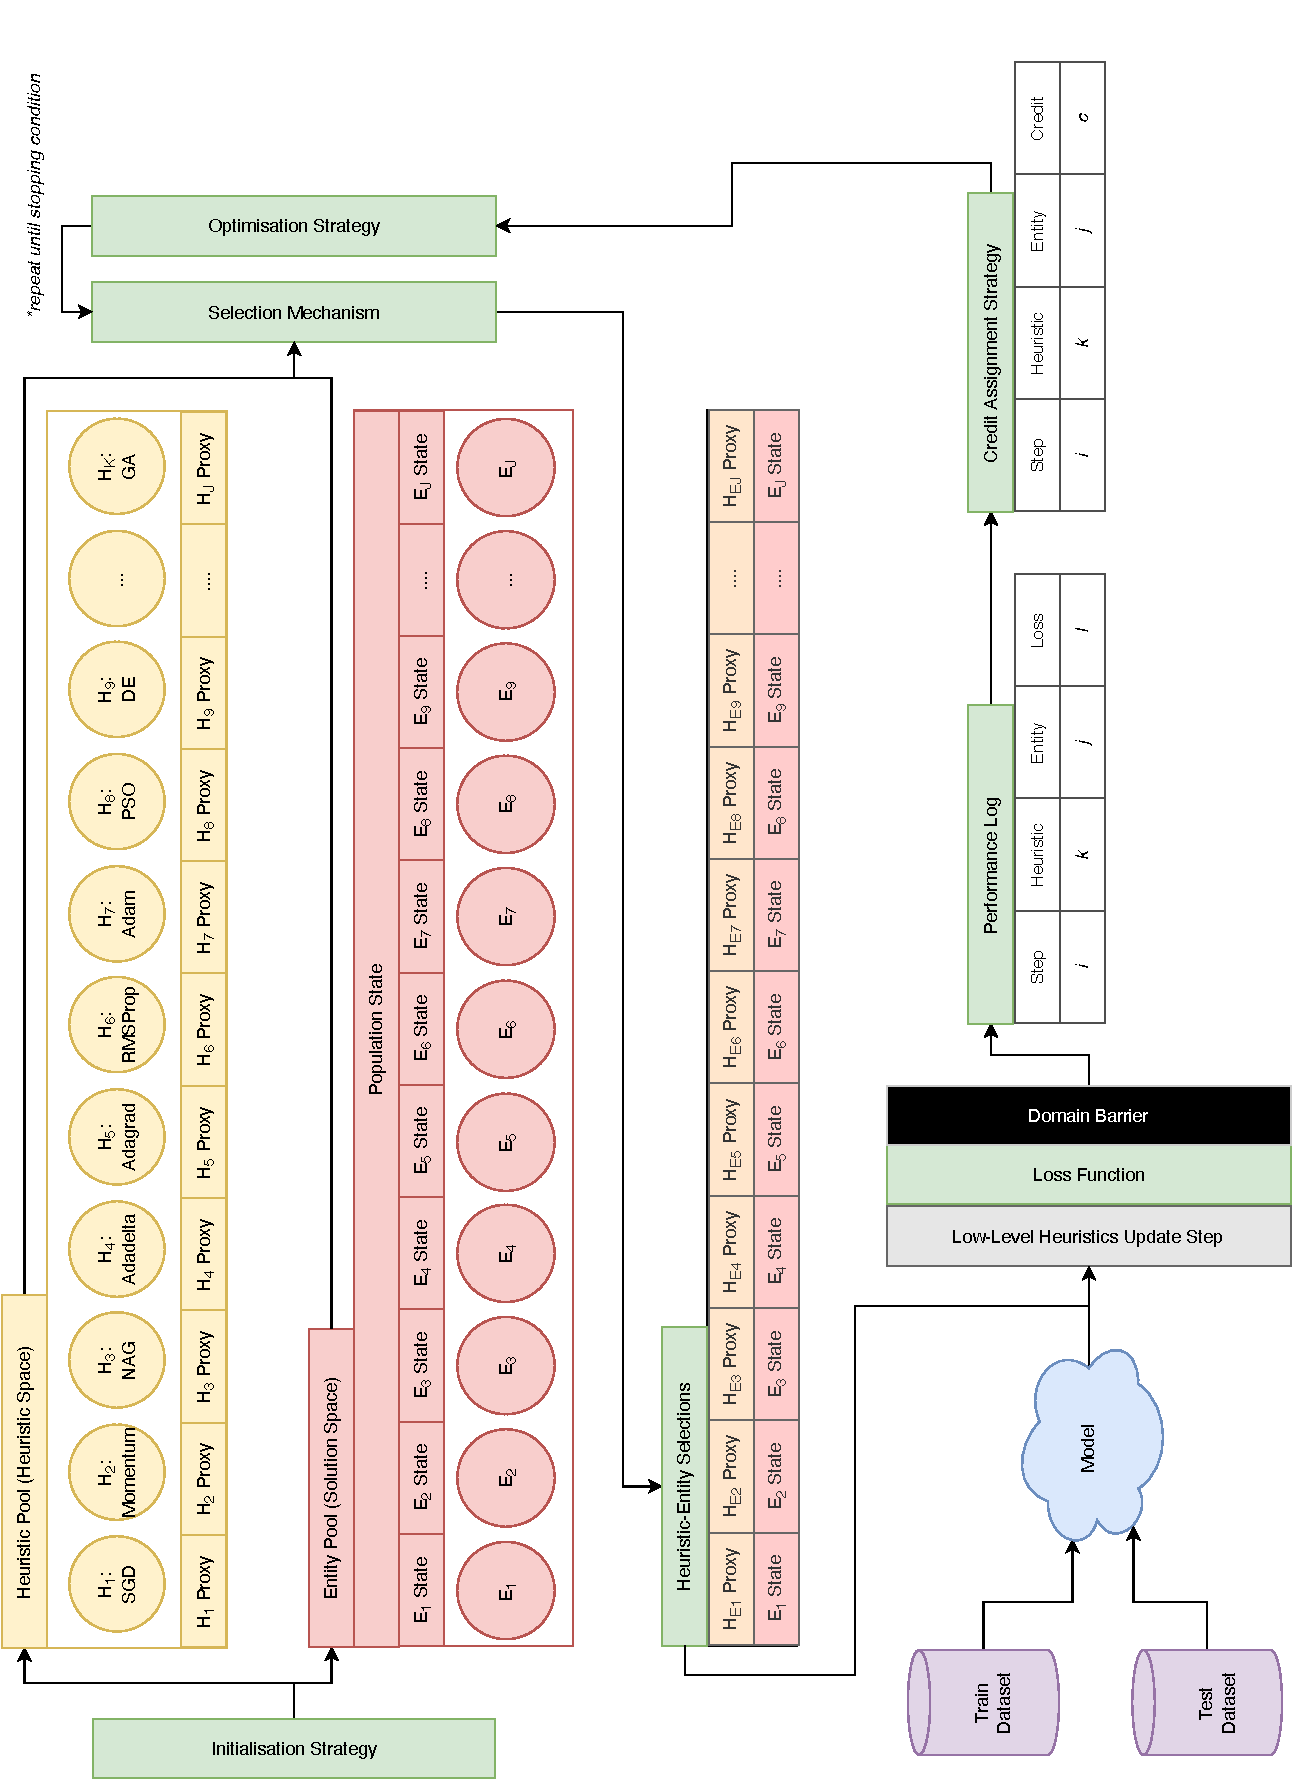
\includegraphics[width=1.0\textwidth]{bhh_architecture.pdf}
      \caption[An illustration of
            the architecture and high level components of the \acf{BHH}.]{An illustration of
            the architecture and high level components of the \acf{BHH}.}
      \label{fig:bhh_architecture}
\end{figure}

With reference to Figure \ref{fig:bhh_architecture}, the components are briefly given below in the order of information flow during the \acs{FFNN} training process steps:

\begin{itemize}
      \item \textbf{Initialisation Step}: The initialisation step refers to the initialisation strategy implemented by the \acs{BHH}.

      \item \textbf{Heuristic Pool}: The \index{heuristic pool}heuristic pool contains a collection of low-level \index{heuristic}heuristics.

      \item \textbf{Entity Pool}: The \index{entity pool}entity pool represents a collection of candidate solutions for the underlying \acs{FFNN}, referred to as entities in a population.

      \item \textbf{Selection Mechanism}: The selection mechanism refers to the Bayesian probabilistic model.

      \item \textbf{Heuristic-Entity Selections}: Every entity in the \index{entity pool}entity pool is assigned a selected heuristic.

      \item \textbf{Train and Test Datasets}: The training set is used to train the model while the test set is used to evaluate the model's generalisation capabilities.

      \item \textbf{Model}: The underlying \acs{FFNN} to be trained.

      \item \textbf{Low-Level Heuristics Update Step}: The low-level heuristics' update step as it applies to its allocated entity.

      \item \textbf{Loss Function}: In supervised learning, the loss function is a measure of distance between predicted output and the ground truth, and is the mechanism used to evaluate the model's performance.

      \item \textbf{Domain Barrier}: The domain barrier is the logical separation of information available in the heuristic space and the solution space. The \acs{BHH} searches in the heuristic space, while low-level heuristics search in the solution space.

      \item \textbf{Performance Log}: Contains a record of heuristic-entity performance at each step of the training process.

      \item \textbf{Credit Assignment Strategy}: The strategy used to assign credit to heuristics for their performance.

      \item \textbf{Update Step}: The high-level heuristic update step as implemented by the \acs{BHH}.
\end{itemize}

\index{heuristic pool}
\section{Heuristic Pool}\label{sec:bhh:heuristic_pool}

Generally speaking, the \index{heuristic pool}heuristic pool is a collection of low-level heuristics under consideration by the \acs{BHH}. The \index{heuristic pool}heuristic pool contains the set of low-level \index{heuristic}heuristics that, together with their performance information, make up the \text{heuristic space}. Importantly, the \acs{BHH} searches in \index{heuristic}heuristic space. The \index{heuristic pool}heuristic pool is defined in terms of the diversity of heuristics, as well as the number of heuristics in the \index{heuristic pool}heuristic pool. Each of these are discussed in the following sections.

\subsection{Heuristic Diversity}\label{sec:bhh:heuristic_pool:diversity}

A \index{heuristic}heuristic's eligibility for inclusion in the \index{heuristic}heuristic pool is determined by its ability to solve the underlying problem and its search behaviour and characteristics. The \index{heuristic pool}heuristic pool should contain a variety of different heuristics that have different search behaviours, so that a trade-off can be made between exploration and exploitation of solutions, as is required during the training process. Heuristics that explore a lot should be selected when exploration is needed, and heuristics that exploit a lot should be selected accordingly. The trade-off between exploration and exploitation is managed by the high-level heuristic. The \acs{BHH} learns to select and apply the appropriate heuristic at the appropriate time, throughout the training process. In doing so, a balance is achieved between exploration and exploitation.

\subsection{Heuristic Pool Size}\label{sec:bhh:heuristic_pool:pool_size}

Another design decision with respect to the heuristic pool is heuristic pool size. Since the \acs{BHH} is a \textit{learning} \acs{HH}, every heuristic that is included in the heuristic pool increases the requirement of more statistical evidence of heuristic performance. Not only does a large \index{heuristic pool}heuristic pool drastically complicate the learning process that is required by the \acs{BHH}, but it also drastically complicates the process of maintaining \textit{state}. State is the term used to describe data that is relevant to the training process, and is maintained between training steps. An example of \textit{local} state is an entity's position, while an example of \textit{global} state is the global best solution found thus far.

\subsection{Proxies}\label{sec:bhh:heuristic:proxies}

The concept of proxies arise from the sparsity of state as maintained by different \index{heuristic}heuristics. Since \index{heuristic}heuristics maintain (possibly) different states, there is an uncertainty of state transition when switching between \index{heuristic}heuristics. Consider an example where the \index{heuristic pool}heuristic pool consists of just two \index{heuristic}heuristics. One heuristic is a gradient-based heuristic that maintains momentum, such as \acs{Adam}~\cite{ref:kingma:2014}. The other is a \index{meta-heuristic}meta-heuristic that does not require a gradient, such as \acs{PSO}~\cite{ref:shi:1998}. Both these \index{heuristic}heuristics track different parameters in their state. For \acs{Adam}, the expected gradient mean and variance is maintained, while the \ac{PSO} maintains record of the gbest and pbest solutions of all of entities. A solution to state indifference is to proxy heuristic state update operations. State is then maintained in two parts:

\begin{itemize}
      \item \textbf{Primary State}: Refers to the state that is originally maintained by a heuristic. The selected heuristic simply applies the normal state update operations to its state.

      \item \textbf{Proxied State}: Refers to the state that is not directly maintained by the heuristic, but can be updated by outsourcing the required state update operation to another heuristic.
\end{itemize}

Primary and proxied state parameters must be maintained together. Since entities represent candidate solutions, which are forms of state, entities are ideal candidates to store and maintain these state parameters. Entities are extended to include the primary state elements of \textit{all} the underlying low-level heuristics, as well as the candidate solution (weights) for the \acs{FFNN}. At each heuristic-entity application step, all state parameters, per entity, are updated either by primary method or by proxied method. The \acs{BHH} thus incorporates a mapping of proxied state update operation as given in the example in Table \ref{tab:bhh:heuristic_pool:proxy_mapping_example}.

\begin{table}[htbp]
      \centering
      \caption{An example of a mapping of proxied state update operation maintained by the \acs{BHH}.}
      \label{tab:bhh:heuristic_pool:proxy_mapping_example}%
      \par\bigskip
      \resizebox{0.38\textwidth}{!}{
            \begin{tabular}{ccccc}
                                                                  &   & \multicolumn{3}{c}{State Parameter}                                                                                                                                                                                      \\
                  \cmidrule{3-5}                                  &   & 1                                                                      & 2                                                                      & 3                                                                      \\
                  \cmidrule{3-5}    \multirow{3}[1]{*}{Heuristic} & A & \cellcolor[rgb]{ .776,  .937,  .808}\textcolor[rgb]{ 0,  .38,  0}{n/a} & \cellcolor[rgb]{ 1,  .922,  .612}\textcolor[rgb]{ .612,  .341,  0}{B}  & \cellcolor[rgb]{ .776,  .937,  .808}\textcolor[rgb]{ 0,  .38,  0}{n/a} \\
                                                                  & B & \cellcolor[rgb]{ .776,  .937,  .808}\textcolor[rgb]{ 0,  .38,  0}{n/a} & \cellcolor[rgb]{ .776,  .937,  .808}\textcolor[rgb]{ 0,  .38,  0}{n/a} & \cellcolor[rgb]{ 1,  .922,  .612}\textcolor[rgb]{ .612,  .341,  0}{A}  \\
                                                                  & C & \cellcolor[rgb]{ .776,  .937,  .808}\textcolor[rgb]{ 0,  .38,  0}{n/a} & \cellcolor[rgb]{ 1,  .922,  .612}\textcolor[rgb]{ .612,  .341,  0}{B}  & \cellcolor[rgb]{ 1,  .922,  .612}\textcolor[rgb]{ .612,  .341,  0}{A}  \\
            \end{tabular}%
      }
\end{table}%

From the example given in Table \ref{tab:bhh:heuristic_pool:proxy_mapping_example}, when \index{heuristic}heuristic A is selected, it will outsource state update operations from \index{heuristic}heuristic B for state parameter 2. Heuristic B will outsource from \index{heuristic}heuristic A for state parameter 3. Finally, \index{heuristic}heuristic C will outsource from \index{heuristic}heuristic A and B for state parameters 2 and 3 respectively. In this way, all \index{heuristic}heuristics maintain all the state parameters.

Proxied state update operations is a simple concept in principle, but requires detailed decomposition of the \index{heuristic}heuristics included in the \index{heuristic pool}heuristic pool. Overlapping and unique state parameters must be identified so that a proxy mapping, such as the one given in Table \ref{tab:bhh:heuristic_pool:proxy_mapping_example}, can be constructed. A suggestion to simplify this process is to borrow concepts from the equations of motion from physics. These include \textit{position}, \textit{velocity}, \textit{acceleration}, and \textit{momentum}. Expressing \index{heuristic}heuristic update steps according to these parameters drastically simplify the process. However, it is possible that \index{heuristic}heuristics implement unique state parameters that do not overlap. These have to be catered for in the proxy mapping.

State parameters and update operations should not be considered in isolation. An example is \textit{position} and \textit{velocity}. Consider, for example, \index{heuristic}heuristics such as \acs{DE}~\cite{ref:price:2006} and \acp{GA}~\cite{ref:holland:1992}. These \index{heuristic}heuristics recombine entities. In the aforementioned case, the concept of an equation of motion does not entirely make sense, since the displacement of its position is not a result of maintaining velocity or momentum, but rather by displacement through recombination. In this particular case, a solution is to apply the recombination operation to \textit{all} applicable state parameters as well, or to nullify the necessary state parameters. Unfortunately, there is no general, automated solution to formulate these heuristic state overlaps. Each \index{heuristic}heuristic must be carefully considered.

\index{entity pool}
\section{Entity Pool}\label{sec:bhh:entity_pool}

The \index{entity pool}entity pool refers to a collection of \textit{entities} that each represent a candidate solution to the underlying \acs{FFNN} being trained. The entities contain information of the solution space. A common naming convention for such a collection is a \textit{population} of entities. The \acs{BHH} is a population-based \acs{HH} and as such, the \index{entity pool}entity pool size or population size is an important design choice. The population size is defined as a hyper-parameter of the \acs{BHH} and can be empirically evaluated.

The \index{entity pool}entity pool maintains two different types of state. These include entity (local) and population (global) state. Each of these are discussed in more detail next.

\subsection{Entity State}\label{sec:bhh:entity_pool:entity_state}

Entities represent candidate solutions to the model's trainable parameters (weights) and other \index{heuristic}heuristic-specific state parameters, as was discussed in Section \ref{sec:bhh:heuristic:proxies}. It can be said that entities implement \textit{local} state. It was mentioned that these entities can be treated as physical \textit{particles} in a hyper-dimensional search environment. Entities model concepts from physics. For example, the candidate solution is represented as the entity's position, and an entity's velocity and acceleration is analogous to the gradient and momentum of the entity respectfully. Examples of entity state parameters, as derived from various low-level \index{heuristic}heuristics, is given as follows:

\begin{itemize}
      \item \textbf{position}: A general parameter that represents the actual candidate solution and is thus a primary state parameter for all \index{heuristic}heuristics.

      \item \textbf{velocity}: Directly implemented by \index{heuristic}heuristics such as \acp{PSO} and is analogous to the gradient for gradient-based \index{heuristic}heuristics such as \ac{Momentum}.

      \item \textbf{gradient}: The last known gradient, as derived from gradient-based \index{heuristic}heuristics.

      \item \textbf{position delta}: The last computed position delta between the current timestep and the previous timestep.

      \item \textbf{sum of the gradients squared}: As required and maintained by \index{heuristic}heuristics such as \acs{Adagrad}.

      \item \textbf{expected position delta variance}: As required and maintained by \index{heuristic}heuristics such as \acs{Adadelta}.

      \item \textbf{expected gradient mean}: As required and maintained by \index{heuristic}heuristics such as \acs{Momentum}, \acs{NAG} and \acs{Adam}.

      \item \textbf{expected gradient variance}: As required and maintained by \index{heuristic}heuristics such as \acs{RMSProp}, \acs{Adadelta} and \acs{Adam}.

      \item \textbf{personal best position}: A parameter that tracks that best known position by the entity thus far, as required and maintained by \index{heuristic}heuristics such as \acs{PSO}.

      \item \textbf{personal best loss}: A parameter that tracks that best known loss by the entity thus far, as required and maintained by \index{heuristic}heuristics such as \acs{PSO}.

      \item \textbf{loss}: A parameter that tracks the loss as achieved by the the entity throughout training.
\end{itemize}

From the list above, it should be clear that entity state becomes increasingly complicated with the increase of the number of distinct \index{heuristic}heuristics in the \index{heuristic pool}heuristic pool with unique state parameters.

\subsection{Population State}\label{sec:bhh:entity_pool:population_state}

The population state refers to a collection of parameters that are shared between the entities in the population. Population state is also referred to as \textit{global} state and represents the population's memory. The population state generally contains state parameters that are of importance to multiple \index{heuristic}heuristics, and usually tracks the state of the population and not individual \index{heuristic}heuristic. Some examples of population state that can arise from different \index{heuristic}heuristics are given below:

\begin{itemize}
      \item \textbf{entities}: Naturally, the population state contains the list of entities in the population.

      \item \textbf{ibest} and \textbf{ibest loss}: Refers to the best position and loss achieved by the population for the current iteration/step.

      \item \textbf{rbest} and \textbf{rbest loss}: Refers to the best position and loss achieved by the population for a number of steps, referred to as the replay window size. The replay window size defines a window of memory for tracking historical performance data of \index{heuristic}heuristics.

      \item \textbf{gbest} and \textbf{gbest loss}: Refers to the overall/global best position and loss achieved by the population for the entire training process. This parameter is introduced by \index{heuristic}heuristics such as \acp{PSO}.
\end{itemize}

Entities in the entity pool are each assigned an associated \index{heuristic}heuristic. The \acs{BHH} selects from the \index{heuristic pool}heuristic pool a low-level \index{heuristic}heuristic to be applied to an individual entity. The outcome of this selection process is a mapping table that tracks which \index{heuristic}heuristic has been selected for which entity. The selection process is executed by the selection mechanism of the \acs{BHH}. These \index{heuristic}heuristic-entity combinations are applied to the underlying \acs{FFNN}. The \acs{BHH} tracks the performance of each of these combinations throughout the training process in a performance log.


\section{Performance Log}\label{sec:bhh:performance_log}

The \acs{BHH} incorporates a form of probabilistic modeling in its selection mechanism. Probability is calculated based on \index{heuristic}heuristic-entity performance over time. Evidence of \index{heuristic}heuristic-entity performance is thus required for the \acs{BHH} to learn. Since the performance log can become very big, only a sliding window of the performance history is maintained at each step in the learning process. The sliding window is also referred to as a \textit{replay} buffer, a term borrowed from the field of \acf{RL}. The replay window size is defined as a hyper-parameter of the \acs{BHH}. The performance log is then simply a table of events and metrics. The \acs{BHH} tracks the following metrics in the performance log:

\begin{itemize}
      \item \textbf{step}: The current mini-batch step.

      \item \textbf{\index{heuristic}heuristic}: The selected heuristic's index.

      \item \textbf{entity}: The entity's index to whom the \index{heuristic}heuristic is applied.

      \item \textbf{loss}: The \index{heuristic}heuristic-entity performance metric. The loss is retrieved from the loss function.

      \item \textbf{ibest loss}: Keeps track of the \textit{iteration} best loss. Thus, the best loss value achieved by all entity-\index{heuristic}heuristic combinations, for a single mini-batch step.

      \item \textbf{rbest loss}:  Keeps track of the \textit{replay} best loss. Thus, the best loss value achieved by all entity-\index{heuristic}heuristic combinations, over all mini-batch steps currently in the performance log/replay window.

      \item \textbf{gbest loss}:  Keeps track of the \textit{global} best loss. Thus, the best loss value achieved by all entity-\index{heuristic}heuristic combinations over all mini-batch steps thus far.
\end{itemize}

An example of the performance log implemented by the \acs{BHH} is given in Table \ref{tab:bhh:performance_log:performance_log_example}.

\begin{table}[htbp]
      \centering
      \caption{An example of the performance log implemented by the \acs{BHH}, showing the first five entities, their allocated \index{heuristic}heuristics and their resulting performance measurements for the first step of the training process.}
      \label{tab:bhh:performance_log:performance_log_example}%
      \par\bigskip
      \resizebox{\textwidth}{!}{
            \begin{tabular}{cccccccc}
                  \textbf{step} & \textbf{entity} & \textbf{heuristic} & \textbf{loss} & \textbf{ibest loss} & \textbf{pbest loss} & \textbf{rbest loss} & \textbf{gbest loss} \\
                  \midrule
                  1             & 1               & 1                  & 0.016444      & 0.016444            & 0.016444            & 0.016444            & 0.016444            \\
                  1             & 2               & 2                  & 0.337965      & 0.016444            & 0.337965            & 0.016444            & 0.016444            \\
                  1             & 3               & 1                  & 0.134781      & 0.016444            & 0.134781            & 0.016444            & 0.016444            \\
                  1             & 4               & 1                  & 0.998719      & 0.016444            & 0.998719            & 0.016444            & 0.016444            \\
                  1             & 5               & 3                  & 0.708702      & 0.016444            & 0.708702            & 0.016444            & 0.016444            \\
            \end{tabular}%
      }
\end{table}%

The performance log itself introduces a number of design considerations as well. The larger the performance log, the longer memory is retained throughout the training process. The performance log size, referred to as the \textit{replay window size}, controls the recency of evidence from which the \acs{BHH} must learn. If the replay window size is too small, it does not accumulate enough samples/evidence to statistically make accurate selections. If the replay window size is too big, a bias could exist for selecting \index{heuristic}heuristics that performed well in the past. Furthermore, it is not guaranteed that past performance is indicative of future performance during the training process. The performance log should be considered along with the selection of a credit assignment strategy.


\section{Credit Assignment Strategy}
\label{sec:bhh:credit_assignment_strategy}

The credit assignment strategy is a mechanism that assigns a discrete credit indicator to \index{heuristic}heuristics that perform well, based on their performance metrics such as loss. The credit assignment strategy implements the ``move acceptance'' process as proposed by~\citeauthor{ref:ozcan:2006}~\cite{ref:ozcan:2006,ref:ozcan:2008} and addresses the credit assignment problem as discussed by~\citeauthor{ref:burke:2010}~\cite{ref:burke:2010}. A good credit assignment strategy will correctly allocate credit to the appropriate \index{heuristic}heuristic-entity combination. The credit assignment strategy to use is defined as a hyper-parameter. The \acs{BHH} implements the following credit assignment strategies to choose from:

\begin{itemize}
      \item \textbf{ibest}: Credit is assigned to the \index{heuristic}heuristic-entity combination that set the \textit{ibest} loss value, meaning that it is the entity-\index{heuristic}heuristic combination that achieved the best performance in the current mini-batch iteration.

      \item \textbf{pbest}: Credit is assigned to the \index{heuristic}heuristic-entity combination that set the \textit{pbest} loss value, meaning that it is the entity-\index{heuristic}heuristic combination that was able to improve on its personal best past performance loss.

      \item \textbf{rbest}: Credit is assigned to the \index{heuristic}heuristic-entity combination that set the \textit{rbest} loss value, meaning that it is the entity-\index{heuristic}heuristic combination that achieved the best performance in the current replay window.

      \item \textbf{gbest}: Credit is assigned to the \index{heuristic}heuristic-entity combination that set the \textit{gbest} loss value, meaning that it is the entity-\index{heuristic}heuristic combination that achieved the overall best performance so far.

      \item \textbf{symmetric}: Credit is assigned to all entity-\index{heuristic}heuristic combinations, regardless of their performance. The symmetric credit assignment strategy does not randomly assign credit, but rather assigns credit to all events. In effect, no learning and performance-bias is achieved with the symmetric credit assignment strategy and thus the symmetric credit assignment strategy is implemented as a basis for comparison. Comparing a credit assignment staretegy to the symmetric credit assignment indicates the ability of the other credit assignment strategy to have an effect on the learning process and performance of the \acs{BHH}.
\end{itemize}

The implementation of a credit assignment strategy is simply a function that translates the performance log from Table \ref{tab:bhh:performance_log:performance_log_example} into Table \ref{tab:bhh:credit_assignment_strategy:credit_assignment_example}.

\begin{table}[htbp]
      \centering
      \caption{Credit assignment strategy output table showing \textit{ibest} credit assignment for the first five entities and their selected heuristics for step 1 of the training process.}
      \label{tab:bhh:credit_assignment_strategy:credit_assignment_example}%
      \par\bigskip
      \resizebox{0.4\textwidth}{!}{
            \begin{tabular}{cccc}
                  \textbf{step} & \textbf{entity} & \textbf{heuristic} & \textbf{credit} \\
                  \midrule
                  1             & 1               & 1                  & true            \\
                  1             & 2               & 2                  & false           \\
                  1             & 3               & 1                  & false           \\
                  1             & 4               & 1                  & false           \\
                  1             & 5               & 3                  & false           \\
            \end{tabular}%
      }
\end{table}%

Credit is used by the selection mechanism of the \acs{BHH}.


\section{Selection Mechanism}\label{sec:bhh:selection_mechanism}

This section provides the detail around the selection mechanism as it is implemented by the \acs{BHH}. Detail is provided around random events as observed by the \acs{BHH}. An argument for independence between random events is made. \index{Bayes' theorem}Bayes' theorem is briefly reviewed in the context of the \acs{BHH} implementation. It is shown how the \acs{BHH} implements a probabilistic, predictive model based on the fundamentals of the Na\"{\i}ve Bayes algorithm. Brief discussions follow on numerical stability and mode collapse.

\subsection{Random Events}
\label{sec:bhh:selection_mechanism:random_events}

Observation of random events is treated as evidence. In the context of a Bayesian approach, this evidence is used to update prior beliefs. The \acs{BHH} distinguishes between the following events:

\begin{itemize}
      \item \textbf{$\boldsymbol{H}$}: The event of observing \textit{heuristics}.
      \item \textbf{$\boldsymbol{E}$}: The event of observing \textit{entities}.
      \item \textbf{$\boldsymbol{C}$}: The event of observing \textit{credit assignments} that indicate that the credit assignment \textit{performance criteria} are met.
\end{itemize}

It should be noted that event information is stored and observed directly from the performance log as presented in Table \ref{tab:bhh:credit_assignment_strategy:credit_assignment_example}. From the above list of events, the event $\boldsymbol{C}$ is dependent on the occurrence of $\boldsymbol{H}$ and $\boldsymbol{E}$ and a credit assignment strategy.

\subsection{Independence}\label{sec:bhh:selection_mechanism:independence}

The dependence between random events can have an impact on the probabilistic model that is implemented. For simplicity, the \acs{BHH} assumes independence between events, although the event $\boldsymbol{C}$ is clearly dependent on the occurrence of $\boldsymbol{H}$ and $\boldsymbol{E}$. Furthermore, the \acs{BHH} assumes independence between steps  and treats each training step as if training has restarted. The \acs{BHH} implements a form of Naïve Bayes classifier, where the appropriate heuristic to assign to an entity is a classification problem. \citeauthor{ref:domingos:1997}~\cite{ref:domingos:1997} mention that although the probability estimates of Bayesian classifiers are only optimal under quadratic loss if the independence assumption holds, the classifier itself can still be optimal under zero-one loss (misclassification rate), even when this assumption is violated by a wide margin. This means that independence can be assumed when the probabilistic model is used as a classifier.

\index{Bayes' theorem}
\subsection{Bayes' Theorem}\label{sec:bhh:selection_mechanism:bayes_theorem}

Chapter \ref{chap:probability} presented \index{Bayes' theorem}Bayes' theorem, but for convenience, it is given below:

\begin{equation}
      \label{eq:bhh:selection_mechanism:bayes_theorem}
      P(A \vert B) = \frac{P(B \vert A)P(A)}{P(B)}
\end{equation}

Since the \acs{BHH} implements a Bayesian classifier, the \acs{BHH} is not concerned with actual probabilities. Equation~\eqref{eq:bhh:selection_mechanism:bayes_theorem} can thus be evaluated for proportionality. The resulting proportionality is expressed as

\begin{equation}
      \label{eq:bhh:selection_mechanism:bayes_theorem_prop_to}
      P(A \vert B) \propto P(B \vert A)P(A)
\end{equation}

The conditionality implemented by \index{Bayes' theorem}Bayes' theorem can be extended to include multiple criteria. \index{Bayes' theorem}Bayes' theorem is used by the selection mechanism of the \acs{BHH}.

\subsection{Predictive Model}\label{sec:bhh:selection_mechanism:predictive_model}

This section presents the predictive model as implemented by the selection mechanism of the \acs{BHH}. The predictive model is arguably the most important component of the \acs{BHH}, because it drives the heuristic selection process. The \acs{BHH} implements a predictive model that predicts which heuristic to select, given the conditionality that a particular entity is used and a particular credit assignment criteria is met. The predictive model can be derived as follows.\\\\
\textbf{Setup}:
\\
Let

\begin{itemize}
      \item $I$ denote the maximum number of instances in the replay window.
      \item $J$ denote the \index{entity pool}entity pool (population) size.
      \item $K$ denote the \index{heuristic pool}heuristic pool size.
      \item $L$ denote the number of credit assignment output classes. Since the output of credit assignment is boolean, $L = 2$.

      \item $\boldsymbol{\alpha} = (\alpha_{1}, \dots, \alpha_{K})$ denote the concentration parameters for the heuristic probability distribution.
      \item $\boldsymbol{\beta} = (\beta_{1}, \dots, \beta_{K})^{J}$ denote the concentration parameters for the entity-heuristic probability distributions.
      \item $\boldsymbol{\gamma} = (\gamma_{1}, \dots, \gamma_{K})^{L}$ denote the concentration parameters for the credit-heuristic probability distribution.

      \item $\boldsymbol{\theta} \vert \boldsymbol{\alpha} \sim Dir(\boldsymbol{\alpha}; K)$ denote the heuristic probability distribution, implementing a \index{Dirichlet probability distribution}Dirichlet probability distribution parameterised by $\boldsymbol{\alpha}$ and $K$. Heuristic selection probabilities are sampled from this distribution.

      \item $\boldsymbol{\phi} \vert \boldsymbol{\beta} \sim Dir(\boldsymbol{\beta}; K)^{J}$ denote the entity-heuristic probability distribution, implementing a \index{Dirichlet probability distribution}Dirichlet probability distribution parameterised by $\boldsymbol{\beta}$ and $K$ for each entity in the \index{entity pool}entity pool with population size $J$. Entity-heuristic probabilities are sampled from this distribution.

      \item $\boldsymbol{\psi} \vert \gamma_{1}, \gamma_{0}  \sim Beta(\gamma_{1}, \gamma_{0})$ denote the credit-heuristic probability distribution, implementing a Beta probability distribution parameterised by $\gamma_{1}$ and $\gamma_{0}$. Credit-heuristic probabilities are sampled from this distribution.

      \item $\boldsymbol{H} \vert \boldsymbol{\theta} \sim Mult(\boldsymbol{\theta}; I, K)$ denote the distribution of heuristics (event $\boldsymbol{H}$), implementing a \index{Multinomial probability distribution}Multinomial distribution, parameterised by the sampled heuristic selection probabilities $\boldsymbol{\theta}$, the \index{heuristic pool}heuristic pool size $K$, and maximum number of instances $I$.

      \item $\boldsymbol{E} \vert \boldsymbol{\phi} \sim Mult(\boldsymbol{\phi}; I, K)^{J}$ denote the distribution of entity-heuristic combinations (event $\boldsymbol{E}$), implementing a \index{Multinomial probability distribution}Multinomial distribution, parameterised by the sampled entity-heuristic selection probabilities $\boldsymbol{\phi}$, the \index{heuristic pool}heuristic pool size $K$, and maximum number of instances $I$ for each entity in $J$.

      \item $\boldsymbol{C} \vert \boldsymbol{\psi} \sim Bin(\boldsymbol{\psi}, I)$ denote the distribution of credit-heuristic combinations (event $\boldsymbol{C}$), implementing a \index{Binomial probability distribution}Binomial probability distribution, parameterised by the sampled credit-heuristic selection probabilities $\boldsymbol{\psi}$ and the maximum number of instances $I$.
\end{itemize}

The parameterised predictive model, as derived from \index{Bayes' theorem}Bayes' theorem, is then given as

\footnotesize
\begin{equation}
      \label{eq:bhh:selection_mechanism:predictive_model}
      \begin{split}
            P(\boldsymbol{H} \vert \boldsymbol{E}, \boldsymbol{C};  \boldsymbol{\theta}, \boldsymbol{\phi}, \boldsymbol{\psi})
            &= \frac{
                  P(\boldsymbol{E}, \boldsymbol{C} \vert \boldsymbol{H};  \boldsymbol{\phi}, \boldsymbol{\psi})  P(\boldsymbol{H} \vert \boldsymbol{\theta})
            }{
                  P(\boldsymbol{E}, \boldsymbol{C} \vert \boldsymbol{\theta}, \boldsymbol{\phi}, \boldsymbol{\psi})
            } \\
            &= \frac{
                  P(\boldsymbol{E} \vert \boldsymbol{H};  \boldsymbol{\phi})  P(\boldsymbol{C} \vert \boldsymbol{H};  \boldsymbol{\psi}) P(\boldsymbol{H} \vert \boldsymbol{\theta})
            }{
                  P(\boldsymbol{E} \vert \boldsymbol{\theta}, \boldsymbol{\psi}) P(\boldsymbol{C} \vert \boldsymbol{\theta}, \boldsymbol{\phi})
            } \\
            &= \frac{
                  P(\boldsymbol{E} \vert \boldsymbol{H};  \boldsymbol{\phi})  P(\boldsymbol{C} \vert \boldsymbol{H};  \boldsymbol{\psi}) P(\boldsymbol{H} \vert \boldsymbol{\theta})
            }{
                  \left[ \sum_{k}^{K} P(\boldsymbol{E}, \boldsymbol{H}=k \vert \boldsymbol{\theta}, \boldsymbol{\phi}) \right] \left[ \sum_{k}^{K}  P(\boldsymbol{C}, \boldsymbol{H}=k \vert \boldsymbol{\theta}, \boldsymbol{\psi}) \right]
            } \\
            &= \frac{
                  P(\boldsymbol{E} \vert \boldsymbol{H};  \boldsymbol{\phi})  P(\boldsymbol{C} \vert \boldsymbol{H};  \boldsymbol{\psi}) P(\boldsymbol{H} \vert \boldsymbol{\theta})
            }{
                  \left[ \sum_{k}^{K} P(\boldsymbol{E} \vert \boldsymbol{H}=k, \boldsymbol{\phi}) P(\boldsymbol{H}=k \vert \boldsymbol{\theta}) \right] \left[ \sum_{k}^{K} P(\boldsymbol{C} \vert \boldsymbol{H}=k, \boldsymbol{\psi}) P(\boldsymbol{H}=k \vert \boldsymbol{\theta}) \right]
            }
      \end{split}
\end{equation}
\normalsize

Notice the joint probability over events $\boldsymbol{E}$ and $\boldsymbol{C}$, given the selection of a heuristic $\boldsymbol{H}$, denoted by the product of the sums of the separate parts for $\boldsymbol{E}$ and $\boldsymbol{C}$, in the denominator. The calculation in the denominator can be intractable. Since the \acs{BHH} selection mechanism uses the predictive model as a classifier, the posterior distribution as given in Equation~\eqref{eq:bhh:selection_mechanism:bayes_theorem} can be evaluated for proportionality as follows:

\begin{equation}
      \label{eq:bhh:selection_mechanism:predictive_model_prop_to}
      \begin{split}
            P(\boldsymbol{H} \vert \boldsymbol{E}, \boldsymbol{C};  \boldsymbol{\theta}, \boldsymbol{\phi}, \boldsymbol{\psi}) &\propto P(\boldsymbol{E} \vert \boldsymbol{H};  \boldsymbol{\phi})  P(\boldsymbol{C} \vert \boldsymbol{H};  \boldsymbol{\psi}) P(\boldsymbol{H} \vert \boldsymbol{\theta})
      \end{split}
\end{equation}

The predictive model thus models the \textit{proportional} probability of the event (selection of) heuristic $\boldsymbol{H}$, given allocation to entity $\boldsymbol{E}$ and credit $\boldsymbol{C}$, parameterised by sampled $\boldsymbol{\theta}$, $\boldsymbol{\phi}$ and $\boldsymbol{\psi}$. These parameters are in turn parameterised by concentrations $\boldsymbol{\alpha}$, $\boldsymbol{\beta}$, $\gamma_{1}$ and $\gamma_{0}$, which denote the prior beliefs of the \acs{BHH}.


\index{Naïve Bayes}
\subsection{Naïve Bayes}\label{sec:bhh:selection_mechanism:naive_bayes}

This section aims to dissect the probabilistic model that is presented in Equestion~\eqref{eq:bhh:selection_mechanism:predictive_model_prop_to}. The \acs{BHH} implements a form of Naïve Bayes classifier, and thus independence between events can be assumed. The following derived \acp{PMF} are provided as fundamental building blocks to show the mechanism by which the \acs{BHH} learns.

The independence between events for class label $\boldsymbol{H}$, simply yields the \ac{PMF} of the \index{Multinomial probability distribution}Multinomial distribution as presented below:

\begin{equation}
      \label{eq:bhh:selection_mechanism:naive_bayes:h_pmf}
      \begin{split}
            P(\boldsymbol{H} \vert \boldsymbol{\theta})
            &\propto \prod_{i=1}^{I} \prod_{k=1}^{K} P(h_{i,k} \vert \theta_{k}) \\
            &\propto \prod_{i=1}^{I} \prod_{k=1}^{K} \theta_{k}^{\mathbbm{1}_{1}(h_{i,k})} \\
            &\propto \prod_{k=1}^{K} \theta_{k}^{\sum_{i=1}^{I} \mathbbm{1}_{1}(h_{i,k})} \\
            &\propto \prod_{k=1}^{K} \theta_{k}^{N_{k}}
      \end{split}
\end{equation}

where $N_{k}$ is a summary variable such that $N_{k} = \sum_{i=i}^{I} \mathbbm{1}_{1}(h_{i,k})$, denoting the count of occurrences of the event $h_{i}$ taking on class $k$ in $I$ independent, identical runs.

The independence between events $\boldsymbol{E}$, given class label $\boldsymbol{H}$, is denoted by the likelihood of $\boldsymbol{E}$, conditional to the occurrence of heuristic $k$ and model parameter $\boldsymbol{\phi}$ as follows:

\begin{equation}
      \label{eq:bhh:selection_mechanism:naive_bayes:EgH_pmf}
      \begin{split}
            P(\boldsymbol{E} \vert \boldsymbol{H};  \boldsymbol{\phi})
            &\propto \prod_{i=1}^{I} \prod_{j=1}^{J} \prod_{k=1}^{K} P(e_{i,j,k} \vert h_{i,k} ; \phi_{j,k})  \\
            &\propto \prod_{i=1}^{I} \prod_{j=1}^{J} \prod_{k=1}^{K} \phi_{j,k}^{\mathbbm{1}_{1}(e_{i,j,k})\mathbbm{1}_{1}(h_{i,k})} \\
            &\propto \prod_{j=1}^{J} \prod_{k=1}^{K} \phi_{j,k}^{ \sum_{i}^{I} \left[ \mathbbm{1}_{1}(e_{i,j,k}) \mathbbm{1}_{1}(h_{i,k}) \right]} \\
            &\propto \prod_{j=1}^{J} \prod_{k=1}^{K} \phi_{j,k}^{N_{j,k}}
      \end{split}
\end{equation}

where $N_{j,k}$ is a summary variable such that $N_{j,k} = \sum_{i=i}^{I} \mathbbm{1}_{1}(e_{i,j,k})\mathbbm{1}_{1}(h_{i,k})$, denoting the count of occurrences of the events $e_{i}$ taking on class $j$ and $h_{i}$ taking on class $k$, i.e. the count of occurrences of both entity $j$ and heuristic $k$ occurring together in $I$ independent, identical runs.

Finally, the independence between events for the performance criteria $\boldsymbol{C}$, given class label $\boldsymbol{H}$, is denoted by the likelihood of $\boldsymbol{C}$, conditional to the occurrence of heuristic $k$ and model parameter $\boldsymbol{\psi}$ as given below:

\begin{equation}
      \label{eq:bhh:selection_mechanism:naive_bayes:CgH_pmf}
      \begin{split}
            P(\boldsymbol{C} \vert \boldsymbol{H}; \boldsymbol{\psi})
            &\propto\prod_{i=1}^{I} \prod_{k=1}^{K} P(c_{i,k} \vert h_{i,k} ; \psi_{k})  \\
            &\propto \prod_{i=1}^{I} \prod_{k=1}^{K} \psi_{k}^{\mathbbm{1}_{1}(c_{i,k})\mathbbm{1}_{1}(h_{i,k})} (1 - \psi_{k})^{\mathbbm{1}_{0}(c_{i,k})\mathbbm{1}_{1}(h_{i,k})}\\
            &\propto \prod_{k=1}^{K} \psi_{k}^{\sum_{i=1}^{I} \mathbbm{1}_{1}(c_{i,k})\mathbbm{1}_{1}(h_{i,k})} (1 - \psi_{k})^{\sum_{i=1}^{I} \mathbbm{1}_{0}(c_{i,k})\mathbbm{1}_{1}(h_{i,k})}\\
            &\propto \prod_{k=1}^{K} \psi_{k}^{N_{1,k}} (1 - \psi_{k})^{N_{0,k}} \\
            &\propto \prod_{k=1}^{K} \psi_{k}^{N_{1,k}} (1 - \psi_{k})^{(N_{k} - N_{1,k})}
      \end{split}
\end{equation}

where $N_{k}$ is the same summary variable as described for Equation~\eqref{eq:bhh:selection_mechanism:naive_bayes:h_pmf}. $N_{1,k}$ is a summary variable such that $N_{1,k} = \sum_{i=1}^{I} \mathbbm{1}_{1}(c_{i,k})\mathbbm{1}_{1}(h_{i,k})$, denoting the count of occurrences of the events $c_{i}$ taking on a success (i.e. $c_{i}=1$) and $h_{i}$ taking on class $k$, i.e. the count of occurrences of both succeeding in the performance criteria and heuristic $k$ occurring together in $I$ independent, identical runs. Similarly, $N_{0,k} = N_{k} - N_{1,k}$ denotes the count of occurrences of the events $c_{i}$ taking on a failure (i.e. $c_{i}=0$) and $h_{i}$ taking on class $k$.

Equations~\eqref{eq:bhh:selection_mechanism:naive_bayes:h_pmf}, \eqref{eq:bhh:selection_mechanism:naive_bayes:EgH_pmf} and \eqref{eq:bhh:selection_mechanism:naive_bayes:CgH_pmf} can be substituded into the proportional evaluation of the predictive model as given in Equation~\eqref{eq:bhh:selection_mechanism:predictive_model_prop_to}, resulting in

\begin{equation}
      \label{eq:bhh:selection_mechanism:naive_bayes:HgEC_pmf}
      \begin{split}
            P(\boldsymbol{H} \vert \boldsymbol{E}, \boldsymbol{C};  \boldsymbol{\theta}, \boldsymbol{\phi}, \boldsymbol{\psi})
            &\propto P(\boldsymbol{E} \vert \boldsymbol{H};  \boldsymbol{\phi})  P(\boldsymbol{C} \vert \boldsymbol{H}; \boldsymbol{\psi}) P(\boldsymbol{H} \vert \boldsymbol{\theta})  \\
            &\propto \left[ \prod_{j=1}^{J} \prod_{k=1}^{K} \phi_{j,k}^{N_{j,k}} \right] \left[ \prod_{k=1}^{K} \psi_{k}^{N_{1,k}} (1 - \psi_{k})^{(N_{k} - N_{1,k})} \right] \left[ \prod_{k=1}^{K} \theta_{k}^{N_{k}} \right]
      \end{split}
\end{equation}

Consider the practical implementation of the predictive model as shown in Equation~\eqref{eq:bhh:selection_mechanism:naive_bayes:HgEC_pmf}. Computationally, the equation presented in Equation~\eqref{eq:bhh:selection_mechanism:naive_bayes:HgEC_pmf} will underflow on a real computer if the resulting probabilities are very small.

\subsection{Numerical Stability}\label{sec:bhh:selection_mechanism:numerical_stability}

When Equation~\eqref{eq:bhh:selection_mechanism:naive_bayes:HgEC_pmf} is evaluated, the numerical stability is shown to underflow if the resulting probabilities from its parts are very small. Multiplication of multiple fractional parameters leads to an even smaller fractional number. Probabilities might be very low at some points during training. Consider an example where training has stagnated, effectively leading to a scenario where a credit assignment strategy never fulfills a credit assignment, yielding an extremely small probability for $\boldsymbol{\psi}$. A solution to the aforementioned problem is to apply the \textit{log-sum-exp} trick. The transformation of Equation~\eqref{eq:bhh:selection_mechanism:naive_bayes:HgEC_pmf} using the log-sum-exp trick is given as

\begin{equation}
      \label{eq:bhh:selection_mechanism:numerical_stability:log_sum_exp}
      \begin{split}
            LSE(P(h_{k} \vert e_{j}, c_{1};  \theta, \phi, \psi)) = \ln(\exp(\phi_{j,k}) +  \exp(\psi_{k}) + \exp(\theta_{k}))
      \end{split}
\end{equation}

The log-sum-exp trick as shown above caters for very small probabilities. However, there might be a situation where a random event is never seen, purely by chance. This results in a scenario referred to as \textit{mode collapse}.

\subsection{Mode Collapse}\label{sec:bhh:selection_mechanism:mode_collapse}

Mode collapse is the situation that occurs where the selective pressure towards a heuristic is close to zero as a result of random sampling, low initial bias, or bad performance. This leads to a situation where the probabilistic model continually decreases the selective pressure, until the selection probability of that heuristic is 0, yielding no further observations of that particular random event. The \acs{BHH} addresses the aforementioned issue by

\begin{itemize}
      \item using \textit{symmetric} initialisation of the concentration parameters $\alpha$, $\beta$, $\gamma_{1}$ and $\gamma_{0}$;

      \item setting the lower-bound of the concentration parameters $\boldsymbol{\alpha}$, $\boldsymbol{\beta}$, $\gamma_{1}$ and $\gamma_{0}$ to 1, so that a selection probability of 0 is highly improbable; and

      \item continuously resampling heuristics throughout the training process, before and after optimisation, eliminating mode collapse as a result of just random sampling.
\end{itemize}

Another suggestion is to ensure that at least one of every heuristic is always selected during training. The \acs{BHH} does not incorporate this approach, because this could result in a situation where a bad choice of heuristic is continually used throughout the training process, possibly resulting in bad update steps/selections. Instead, the \acs{BHH} relies on the underlying learning process to control the selective pressure according to performance and nothing else. If this leads to a situation where mode collapse occurs, the \acs{BHH} accepts the outcome.

\section{Optimisation Step}\label{sec:bhh:optimisation_step}

Thus far all the fundamental components of the \acs{BHH} have been presented. The final step that is missing is to present the optimisation step by which the learning process takes place. This section provides a solid mathematical explanation to show exactly how the \acs{BHH} is able to learn. This section provides a brief overview of the role of concentration parameters and pseudo counts. Detailed discussions and mathematical descriptions follow for two techniques, known as \acs{MLE} and \acs{MAP}, that are used to train Na\"{\i}ve Bayes classifiers.

\subsection{Concentration Parameters and Pseudo Counts}\label{sec:bhh:optimisation_step:concentration_pseudo_counts}

The intent of the \acs{BHH} is to gather evidence that can be used to update prior beliefs about which heuristics perform well during training. These beliefs are represented by the concentration parameters $\boldsymbol{\alpha}$, $\boldsymbol{\beta}$, $\gamma_{1}$ and $\gamma_{0}$. A change in prior beliefs is represented by a change in these concentration parameters. Specifically, it can be said that the optimisation process implemented by the \acs{BHH} updates \textit{pseudo counts} of events that are observed in the performance logs. These pseudo counts track the occurrence of a heuristic, an entity, and resulting performance of these two elements. Through the credit assignment strategy, these pseudo counts are biased towards entity-heuristic combinations that meet performance requirements and yield credit allocations.

The \acs{BHH} is an adaptive \ac{HH}, meaning that it implements online learning. Online learning refers to a process where learning happens during the training process. Throughout the training process, concentration parameters are updated strategically to guide the selection mechanism towards heuristics that perform well. The learning capability of the \acs{BHH} lies in carefully updating these concentration parameters. Another possibility is to introduce \textit{a priori} information in the form of expert knowledge. A priori biases can be introduced by carefully setting the concentration parameters to values that are known to be good.

Generally, there are two different techniques that are used to train Naïve Bayes classifiers. The frequentist approach implements \acf{MLE} and the Bayesian approach implements \acf{MAP}. These methods are provided in Sections \ref{sec:bhh:optimisation_step:mle} and \ref{sec:bhh:optimisation_step:map} respectively and show how the concentration parameters are updated throughout the training process, yielding the mechanism by which optimisation and learning takes place. It should be mentioned that the \acs{BHH} makes use of \acs{MAP} to optimise the predictive model. However, the details of \acs{MLE} is provided as well as it contains fundamental mathematical building blocks that are required to present \acs{MAP}.


\index{maximum likelihood estimation}
\subsection{Maximum Likelihood Estimation}\label{sec:bhh:optimisation_step:mle}

In probability theory and statistics, \acf{MLE} is a method that estimates the parameters of a prior probability distribution given newly observed data and evidence. This section shows that the values for $\boldsymbol{\theta}$, $\boldsymbol{\phi}$ and $\boldsymbol{\psi}$ can be estimated by \acs{MLE} as follows:

\begin{equation}
      \label{eq:bhh:optimisation_step:mle:theta}
      \begin{split}
            \hat{\theta}_{k} = E[\theta_{k}] = \frac{N_{k}}{N}
      \end{split}
\end{equation}

\begin{equation}
      \label{eq:bhh:optimisation_step:mle:phi}
      \begin{split}
            \hat{\phi}_{j,k} = E[\phi_{j,k}] = \frac{N_{j,k}}{N_{j}}
      \end{split}
\end{equation}

\begin{equation}
      \label{eq:bhh:optimisation_step:mle:psi}
      \begin{split}
            \hat{\psi}_{k} = E[\psi_{k}] = \frac{N_{1,k}}{N_{k}}
      \end{split}
\end{equation}

The derivations of the \acs{MLE} for $\hat{\theta}_{k}$, $\hat{\phi}_{j,k}$ and
$\hat{\psi}_{k}$ are presented as follows: The log likelihood of $\boldsymbol{\hat{\theta}}$, $\boldsymbol{\hat{\phi}}$ and $\boldsymbol{\hat{\psi}}$ as derived from the Equation~\eqref{eq:bhh:selection_mechanism:predictive_model_prop_to} is given as

\begin{equation}
      \label{eq:bhh:optimisation_step:mle:log_likelihood_all}
      \begin{split}
            & \mathcal{L}(\boldsymbol{\theta}, \boldsymbol{\phi}, \boldsymbol{\psi}) \\
            &= \ln\left(\left[ \prod_{j=1}^{J} \prod_{k=1}^{K} \phi_{j,k}^{N_{j,k}} \right] \left[ \prod_{k=1}^{K} \psi_{k}^{N_{1,k}} (1 - \psi_{k})^{(N_{k} - N_{1,k})} \right] \left[ \prod_{k=1}^{K} \theta_{k}^{N_{k}} \right] \right) \\
            &= \ln \left( \prod_{j=1}^{J} \prod_{k=1}^{K} \phi_{j,k}^{N_{j,k}} \right) +  \ln \left( \prod_{k=1}^{K} \psi_{k}^{N_{1,k}} (1 - \psi_{k})^{(N_{k} - N_{1,k})} \right) + \ln \left( \prod_{k=1}^{K} \theta_{k}^{N_{k}} \right) \\
            &= \left( \sum_{j=1}^{J} \sum_{k=1}^{K} N_{j,k} \ ln \left( \phi_{j,k}
            \right) \right) \\
            &+ \left( \sum_{k=1}^{K} N_{1,k} \ln \left( \psi_{k} \right) + \left( N_{k} - N_{1,k} \right) \ln \left( 1 - \psi_{k} \right) \right) + \left( \sum_{k=1}^{K} N_{k} \ln \left( \theta_{k} \right) \right)
      \end{split}
\end{equation}

Equation~\eqref{eq:bhh:optimisation_step:mle:log_likelihood_all} is broken down into each of its components. Consider the log likelihood of $\boldsymbol{\psi}$ as denoted by

\begin{equation}
      \label{eq:bhh:optimisation_step:mle:log_likelihood_psi}
      \begin{split}
            \mathcal{L}(\boldsymbol{\psi}) &=  \sum_{k=1}^{K} N_{1,k} \ln \left( \psi_{k} \right) + \left( N_{k} - N_{1,k} \right) \ln \left( 1 - \psi_{k} \right)
      \end{split}
\end{equation}

The \acs{MLE} for $\hat{\psi_{k}} $ is calculated by taking the partial derivative of Equation~\eqref{eq:bhh:optimisation_step:mle:log_likelihood_psi} with respect to $\psi_{k}$ and equating to zero as follows:

\begin{equation}
      \label{eq:bhh:optimisation_step:mle:proof_log_likelihood_psi}
      \begin{split}
            \frac{\partial \mathcal{L}(\boldsymbol{\psi})}{\partial \psi_{k}} &= N_{1,k} \frac{1}{ \psi_{k}} + \left( N_{k} - N_{1,k} \right) \frac{-1}{ \left( 1 - \psi_{k} \right) } \\
            \therefore 0 &=  \frac{ N_{1,k} \left( 1 - \psi_{k} \right) +  \left( N_{1,k} - N_{k} \right) \psi_{k}}{ \psi_{k} \left( 1 - \psi_{k} \right) } \\
            \therefore 0 &=  N_{1,k} \left( 1 - \psi_{k} \right) +  \left( N_{1,k} - N_{k} \right) \psi_{k} \\
            \therefore 0 &=  N_{1,k} - N_{1,k} \psi_{k}  +  N_{1,k} \psi_{k} - N_{k}\psi_{k} \\
            \therefore 0 &=  N_{1,k} - N_{k}\psi_{k} \\
            \therefore N_{k}\psi_{k} &=  N_{1,k} \\
            \therefore \hat{\psi}_{k} &=  \frac{N_{1,k}}{N_{k}} \\
      \end{split}
\end{equation}

The \acs{MLE} for $\hat{\theta_{k}} $ can be calculated similarly. However, the $K-1$ simplex $S$ has to be compensated for by adding error factor, $\epsilon$, to correct values for $\boldsymbol{\theta}$, where $\sum_{k}^{K} \theta_{k} \neq 1$. The new log likelihood function is then given as

\begin{equation}
      \label{eq:bhh:optimisation_step:mle:proof_log_likelihood_theta_part_1}
      \begin{split}
            \mathcal{L}(\boldsymbol{\theta}, \epsilon)
            &=  \left( \sum_{k=1}^{K} N_{k} \ln \left( \theta_{k} \right) \right) + \epsilon \left( 1 - \sum_{k=1}^{K} \theta_{k} \right) \\
            &=  \left( \sum_{k=1}^{K} N_{k} \ln \left( \theta_{k} \right) \right) + \left( \epsilon -  \epsilon \sum_{k=1}^{K} \theta_{k} \right)
      \end{split}
\end{equation}

Solving first for $\epsilon$ yields

\begin{equation}
      \label{eq:bhh:optimisation_step:mle:proof_log_likelihood_theta_part_2}
      \begin{split}
            \frac{\partial \mathcal{L}(\boldsymbol{\theta}, \epsilon)}{\partial \epsilon} &= 1 - \sum_{k=1}^{K} \theta_{k}  \\
            \therefore \sum_{k=1}^{K} \theta_{k}  &= 1
      \end{split}
\end{equation}

Then solving for $\theta_{k}$ yields

\begin{equation}
      \label{eq:bhh:optimisation_step:mle:proof_log_likelihood_theta_part_3}
      \begin{split}
            \frac{\partial \mathcal{L}(\boldsymbol{\theta}, \epsilon)}{\partial \theta_{k}} &=  N_{k} \frac{1}{\theta_{k}}  + \epsilon(-1) \\
            \therefore \frac{N_{k}}{\theta_{k}} &= \epsilon \\
            \therefore N_{k} &= \theta_{k} \epsilon \\
            \therefore \sum_{k=1}^{K} N_{k} &= \sum_{k=1}^{K} \theta_{k} \epsilon \\
            \therefore N &= \epsilon \sum_{k=1}^{K} \theta_{k} \\
            \therefore N &= \epsilon
      \end{split}
\end{equation}

Substitution of $N = \epsilon$ back into Equation~\eqref{eq:bhh:optimisation_step:mle:proof_log_likelihood_theta_part_3} yields

\begin{equation}
      \label{eq:bhh:optimisation_step:mle:proof_log_likelihood_theta_part_4}
      \begin{split}
            N_{k} &= \theta_{k} \epsilon \\
            N_{k} &= \theta_{k} N \\
            \hat{\theta}_{k} &= \frac{N_{k}}{N}\\
      \end{split}
\end{equation}

The \acs{MLE} for $\hat{\phi}_{j, k} $ is calculated similarly. To compensate for the $K-1$ simplex $S$, an error, $\boldsymbol{\lambda} = (\lambda_{1}, \dots, \lambda_{J})$ is added as follows:

\begin{equation}
      \label{eq:bhh:optimisation_step:mle:proof_log_likelihood_phi_part_1}
      \begin{split}
            \mathcal{L}(\boldsymbol{\phi}, \boldsymbol{\lambda})
            &=  \left( \sum_{j=1}^{J} \sum_{k=1}^{K} N_{j,k} \ ln \left( \phi_{j,k} \right) \right) + \sum_{j=1}^{J} \lambda_{j} \left( 1 - \sum_{k=1}^{K} \phi_{j,k} \right) \\
            &=  \left( \sum_{j=1}^{J} \sum_{k=1}^{K} N_{j,k} \ ln \left( \phi_{j,k} \right) \right) + \sum_{j=1}^{J} \lambda_{j} - \sum_{j=1}^{J} \lambda_{j} \sum_{k=1}^{K} \phi_{j,k} \\
      \end{split}
\end{equation}

Solving first for $\lambda_{j}$ yields

\begin{equation}
      \label{eq:bhh:optimisation_step:mle:proof_log_likelihood_phi_part_2}
      \begin{split}
            \frac{\partial \mathcal{L}(\boldsymbol{\phi}, \boldsymbol{\lambda})}{\partial \lambda_{j}} &= 1 - \sum_{k=1}^{K} \phi_{j,k}  \\
            \therefore \sum_{k=1}^{K} \phi_{j,k}  &= 1
      \end{split}
\end{equation}

Then solving for $\phi_{j,k}$ yields

\begin{equation}
      \label{eq:bhh:optimisation_step:mle:proof_log_likelihood_phi_part_3}
      \begin{split}
            \frac{\partial \mathcal{L}(\boldsymbol{\phi}, \boldsymbol{\lambda})}{\partial \phi_{j,k}} &= N_{j,k} \frac{1}{\phi_{j,k}}  - \lambda_{j} \\
            \therefore \frac{N_{j,k}}{\phi_{jk}} &= \lambda_{j} \\
            \therefore N_{j,k} &= \phi_{j,k} \lambda_{j} \\
            \therefore \sum_{k=1}^{K} N_{j,k} &= \sum_{k=1}^{K} \phi_{j,k} \lambda_{j} \\
            \therefore N_{j} &= \lambda_{j} \sum_{k=1}^{K} \phi_{j,k} \\
            \therefore N_{j} &= \lambda_{j}
      \end{split}
\end{equation}

Substitution of $N_{j} = \lambda_{j}$ back into Equation~\eqref{eq:bhh:optimisation_step:mle:proof_log_likelihood_phi_part_3} yields

\begin{equation}
      \label{eq:bhh:optimisation_step:mle:proof_log_likelihood_phi_part_4}
      \begin{split}
            N_{j,k} &= \phi_{j,k} \lambda_{j} \\
            N_{j,k} &= \phi_{j,k} N_{j} \\
            \hat{\phi}_{j,k} &= \frac{N_{j,k}}{N_{j}}\\
      \end{split}
\end{equation}

\index{maximum a posteriori estimation}
\subsection{Maximum A Posteriori Estimation}\label{sec:bhh:optimisation_step:map}

Another approach to optimise the values for $\hat{\theta}_{k}$, $\hat{\phi}_{j,k}$ and $\hat{\psi}_{k}$ is to optimise the parameters by their probability distributions' parameters. This process is referred to as \index{Bayesian analysis}\textit{Bayesian analysis}. This section provides the mathematical details of Bayesian analysis and \acf{MAP} as it is implemented in the \acs{BHH}.

Bayesian analysis makes use of the \textit{posterior} probability distribution. The posterior distribution is simply expressed proportionally as

\begin{equation}
      \label{eq:bhh:optimisation_step:map:bayesian_analysis_lamens}
      \begin{split}
            POSTERIOR \propto LIKELIHOOD \times PRIOR
      \end{split}
\end{equation}

The event $\boldsymbol{H}$ is a multinomial distribution with probability parameter $\boldsymbol{\theta}$. It is known that the conjugate prior to a multinomial distribution is a \index{Dirichlet probability distribution}Dirichlet probability distribution. The \textit{prior} probability distribution for $\boldsymbol{\theta}$ is thus presented as

\begin{equation}
      \label{eq:bhh:optimisation_step:map:map_theta_prior}
      \begin{split}
            P(\boldsymbol{\theta} | \boldsymbol{\alpha})
            &\propto \prod_{k=1}^{K} \theta_{k}^{\alpha_{k} -1}
      \end{split}
\end{equation}

Furthermore, the event $\boldsymbol{E}$ is also a multinomial distribution with parameter $\boldsymbol{\phi}$. The \textit{prior} probability distribution for $\boldsymbol{\phi}$ is thus presented as

\begin{equation}
      \label{eq:bhh:optimisation_step:map:map_phi_prior}
      \begin{split}
            P(\boldsymbol{\phi} \vert \boldsymbol{\beta})
            &\propto \prod_{j=1}^{J}  \prod_{k=1}^{K} \phi_{j,k}^{\beta_{j,k} -1}
      \end{split}
\end{equation}

Finally, the event $\boldsymbol{C}$ is a \index{Binomial probability distribution}Binomial probability distribution with probability parameter $\boldsymbol{\psi}$. It is known that the conjugate prior to a \index{Binomial probability distribution}Binomial probability distribution is a Beta probability distribution. The prior probability distribution for $\boldsymbol{\psi}$ is thus presented as

\begin{equation}
      \label{eq:bhh:optimisation_step:map:map_psi_prior}
      \begin{split}
            P(\boldsymbol{\psi} | \gamma_{1}, \gamma_{0})
            &\propto \prod_{k=1}^{K} \psi_{k}^{\gamma_{1,k}} (1- \psi_{k})^{\gamma_{2,k}}
      \end{split}
\end{equation}

Putting the likelihood and priors together yields the posterior distribution as given below:

\footnotesize
\begin{equation}
      \label{eq:bhh:optimisation_step:map:posterior}
      \begin{split}
            P(\boldsymbol{\theta}, \boldsymbol{\phi}, \boldsymbol{\psi} \vert \boldsymbol{H}, \boldsymbol{E}, \boldsymbol{C};  \boldsymbol{\alpha}, \boldsymbol{\beta}, \gamma_{1}, \gamma_{0})
            &\propto P(\boldsymbol{H} \vert \boldsymbol{E}, \boldsymbol{C}; \boldsymbol{\theta}, \boldsymbol{\phi}, \boldsymbol{\psi})P(\boldsymbol{\theta}, \boldsymbol{\phi}, \boldsymbol{\psi} \vert \boldsymbol{\alpha}, \boldsymbol{\beta}, \gamma_{1}, \gamma_{0}) \\
            &= P(\boldsymbol{E} \vert \boldsymbol{H}; \boldsymbol{\phi}) P(\boldsymbol{C} \vert \boldsymbol{H}; \boldsymbol{\psi}) P(\boldsymbol{H} \vert \boldsymbol{\theta}) P(\boldsymbol{\phi} \vert \boldsymbol{\beta}) P(\boldsymbol{\psi} \vert \gamma_{1}, \gamma_{0}) P(\boldsymbol{\theta} \vert \boldsymbol{\alpha})  \\
            &= \left[ \prod_{j=1}^{J} \prod_{k=1}^{K} \phi_{j,k}^{N_{j,k}} \right] \left[ \prod_{k=1}^{K} \psi_{k}^{N_{1,k}} (1 - \psi_{k})^{(N_{k} - N_{1,k})} \right] \left[ \prod_{k=1}^{K} \theta_{k}^{N_{k}} \right] \\
            &\times \left[ \prod_{j=1}^{J} \prod_{k=1}^{K} \phi_{j,k}^{\beta_{j,k} - 1} \right] \left[ \prod_{k=1}^{K} \psi_{k}^{\gamma_{1,k} - 1} (1 - \psi_{k})^{\gamma_{2,k} - 1} \right] \\
            &\times \left[ \prod_{k=1}^{K} \theta_{k}^{\alpha_{k} - 1} \right] \\
            &= \left[ \prod_{j=1}^{J} \prod_{k=1}^{K} \phi_{j,k}^{(N_{j,k} + \beta_{j,k}) - 1} \right] \\
            &\times \left[ \prod_{k=1}^{K} \psi_{k}^{(N_{1,k} + \gamma_{1,k}) - 1} (1 - \psi_{k})^{(N_{0,k} + \gamma_{2,k} )- 1} \right] \\
            &\times \left[ \prod_{k=1}^{K} \theta_{k}^{(N_{k} + \alpha_{k}) - 1} \right]
      \end{split}
\end{equation}
\normalsize

From Equation~\eqref{eq:bhh:optimisation_step:map:posterior} above, it can be seen that the posterior distribution has the same form, $\mathcal{A}(v)$, as the prior distribution. The concentration update operations are then be given as

\begin{equation}
      \label{eq:bhh:optimisation_step:map:alpha_update_operation}
      \begin{split}
            \alpha_{k}(t+1) = N_{k} + \alpha_{k}(t)
      \end{split}
\end{equation}

\begin{equation}
      \label{eq:bhh:optimisation_step:map:beta_update_operation}
      \begin{split}
            \beta_{j,k}(t+1) = N_{j,k} + \beta_{j,k}(t)
      \end{split}
\end{equation}

\begin{equation}
      \label{eq:bhh:optimisation_step:map:gamma1_update_operation}
      \begin{split}
            \gamma_{1,k}(t+1) = N_{1,k} + \gamma_{1,k}(t)
      \end{split}
\end{equation}

\begin{equation}
      \label{eq:bhh:optimisation_step:map:gamma2_update_operation}
      \begin{split}
            \gamma_{2,k}(t+1) = N_{0,k} + \gamma_{2,k}(t)
      \end{split}
\end{equation}

It can be seen that the prior and posterior probability distributions are of the same form, $\mathcal{A}(v)$. It can therefore be said that the \acs{BHH} implements a Gaussian process~\cite{ref:gortler:2019}. Since the reselection of heuristics happens at regular intervals, the outcome of a selection in one iteration may influence the outcome of another in the next iteration, making the implementation of the \acs{BHH} a \acs{HMM}~\cite{ref:rabiner:1986}.


\section{Hyper-Parameters}\label{sec:bhh:hyper_parameters}

This section provides a breakdown of all the hyper-parameters that were identified and briefly mentioned in this chapter. The following hyper-parameters are presented: \index{heuristic pool}\textit{heuristic pool}, \textit{population size}, \textit{credit assignment strategy}, \textit{reselection interval}, \textit{replay window size}, \textit{reanalysis interval}, \textit{burn in window size}, \textit{discounted rewards} and \textit{normalisation}. Some logical arguments can be made as to what their values should be. However it is still up to empirical analysis to determine the effects of certain hyper-parameter design decisions. Where possible, a range of possible values are provided.

\index{heuristic pool}
\subsection{Heuristic Pool}\label{sec:bhh:hyper_parameters:heuristic_pool}

Section \ref{sec:bhh:heuristic_pool} provided the reader with the context and detail of the \index{heuristic pool}heuristic pool as it is included in the architecture of the \acs{BHH}. A detailed discussion was given around the importance of diversity and balancing exploration and exploitation capabilities. The \index{heuristic pool}heuristic pool hyper-parameter refers to the heuristic-pool configuration that is used. The configuration of the \index{heuristic pool}heuristic pool should account for the following factors:

\begin{itemize}
      \item The type of low-level heuristics to include in the \index{heuristic pool}heuristic pool. This dissertation investigates two main groups, including gradient-based \index{heuristic}heuristics and \acp{MH}.

      \item The low-level heuristics' hyper-parameters. At a lower-level, each of these heuristics have their own set of hyper-parameters.

      \item The \index{heuristic pool}heuristic pool size. This refers to the number of heuristics in the \index{heuristic pool}heuristic pool.
\end{itemize}

The design choices at a high level are not as strict for the \acs{BHH} as it is for low-level heuristics. If the choice of hyper-parameters is uncertain, multiple configurations of a low-level heuristic, each with its own unique hyper-parameter configurations, can be included in the \index{heuristic pool}heuristic pool.

\subsection{Population Size}\label{sec:bhh:hyper_parameters:population_size}

Population size refers to the number of entities included in the \index{entity pool}entity pool. The population size to use is to be determined empirically. Naturally, an assumption is made that a larger population could lead to better results, assuming that entities are initialised uniformly across the solution search space. However, larger population sizes are computationally more expensive. \citeauthor{ref:oldewage:2017}~\cite{ref:oldewage:2017} mentions that a large number of particles (entities) may be able to traverse a greater portion of the search space, because every particle provides additional information about the search space. However, it is to be determined if this is indeed the case for the \acs{BHH}. The following factors need to be considered when picking a population size:

\begin{itemize}
      \item When considering the lower bound of possible population sizes, take into account the highest, minimum population size required by all low-level \index{heuristic}heuristics. For example, if \Acs{DE} is included into the \index{heuristic}heuristic pool, a population size of at least four is required. For \acs{PSO}, the minimum population size is three.

      \item When considering the upper bound of possible population sizes, take into account that a bigger population size results in a more computationally expensive training process. Furthermore, there could exist a point of \textit{diminishing returns} where an increase in population size does not yield any better outcome.
\end{itemize}

\subsection{Credit Assignment Strategy}\label{sec:bhh:hyper_parameters:credit}

Five different credit assignment strategies were presented in Section \ref{sec:bhh:credit_assignment_strategy}. The choice of credit assignment is assumed to be problem dependent. However, this is to be tested empirically. Along with the credit assignment strategy itself, the following factors related to the credit assignment strategy should be considered:

\begin{itemize}
      \item When to apply credit assignment during the training process.
      \item What should the credit assignment score/value be (default = 1).
      \item To what degree should credit assignment be allocated to past results in the performance log.
\end{itemize}

A number of other hyper-parameters are specifically included to address the list of considerations as given above. These include the \textit{reselection interval}, \textit{replay window size} and \textit{reanalysis interval}, \textit{burn in window size}, \textit{discounted rewards} and \textit{normalisation}.

\subsection{Reselection Interval}\label{sec:bhh:hyper_parameters:reselection}

The reselection interval is a hyper-parameter that controls how often heuristic selections are resampled from the heuristic distribution, parameterised by the heuristic selection probability that is learnt. The choice of reselection should be influenced by the following considerations: If reselection happens too frequently, heuristics are not allowed sufficient time to achieve their goals and to smooth out update steps. If reselection happens too infrequently, it does not allow for sufficient collection of samples/evidence from which learning is done. Naturally, the correct reselection interval to use is to be determined empirically.

\subsection{Replay Window Size}\label{sec:bhh:hyper_parameters:replay}

The replay window size is a hyper-parameter that controls how much historical performance information is kept in the performance log for the \acs{BHH} to learn from and was introduced in Section \ref{sec:bhh:performance_log}. The replay window size is a parameter that is borrowed from \acf{RL} and aims to control the effect that past performances have on the \acs{BHH}. A replay window size that is too small includes little to no memory, resulting in a situation where the \acs{BHH} simply looks at the most recent evidence that is collected and nothing more. On the contrary, if the replay window size is large, the \acs{BHH} tracks a longer history of past performances, leading to a situation where previously well-performing heuristics that are not relevant later in the training process, are still selected often.

\subsection{Reanalysis Interval}\label{sec:bhh:hyper_parameters:reanalysis}

The reanalysis interval is a hyper-parameter that controls how often the \acs{BHH} updates its past beliefs (priors). The reanalysis interval goes hand in hand with the reselection interval and replay window size. If the reanalysis interval is too small, the \acs{BHH} prematurely updates its priors. Similar to other hyper-parameters discussed thus far, the correct value to use for the reanalysis interval is to be determined empirically. However, some logical exclusions can be made. A reanalysis interval that is smaller than the reselection interval does not make sense, since the effects of reanalysis are only realised during reselection. A reanalysis interval that is too big could lead to a situation where the delay in updating priors could be detrimental to the outcomes of the \acs{BHH}.

\subsection{Burn In}\label{sec:bhh:hyper_parameters:burn_in}

Burn in is a hyper-parameter that is borrowed from \acf{MCMC} and aims to delay the learning process of the \acs{BHH}. The intent of the burn in hyper-parameter is to determine if heuristics need time to execute before reanalysis starts. Notice that a delay in the learning process does not mean that reselection does not occur or that performance information is not collected in the replay window. Therefore, it should be noted that the burn in window size, reselection interval, replay window size, and reanalysis interval should be considered together. If the replay window size is smaller than the burn in window size, performance information is discarded and an opportunity to learn is lost.

\index{discounted rewards}
\subsection{Discounted Rewards}\label{sec:bhh:hyper_parameters:discounted_rewards}

\index{discounted rewards}Discounted rewards is another hyper-parameter that is borrowed from \acs{RL} and is a flag that determines if discounted rewards are applied or not. \index{discounted rewards}Discounted rewards refer to an implementation where credit assignments for past performances are exponentially decreased further into the past. An exponential decay factor of 0.5 is proposed. The intent of the discounted rewards flag is to scale the effect of past performances that are further back in the performance log, such that they have a smaller impact than more recent evidence on the learning process of the \acs{BHH}.

\subsection{Normalisation}\label{sec:bhh:hyper_parameters:normalisation}

Normalisation is a hyper-parameter that provides a mechanism of control for the degree to which exploration is allowed. Figure \ref{sec:bhh:hyper_parameters:discounted_rewards:normalisation} shows the effect of different concentrations ($\alpha$ and $\beta$) on the Beta probability distribution. By normalising the concentration parameters for the \acs{BHH} ($\boldsymbol{\alpha}$, $\boldsymbol{\beta}$, $\gamma_{1}$ and $\gamma_{0}$), the variance of the selection probability distributions increases, allowing for sampled probabilities further from the mean and thus allowing for more exploration.

\begin{figure}[htb]
      \begin{subfigure}{0.49\textwidth}
            \centering
            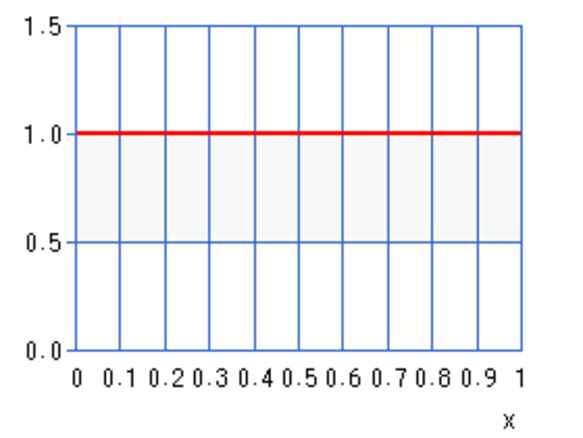
\includegraphics[width=\textwidth]{images/beta_1_1.pdf}
            \caption{$\alpha=1$, $\beta=1$}
            \label{sec:bhh:hyper_parameters:normalisation_beta_1_1}
      \end{subfigure}
      \begin{subfigure}{0.49\textwidth}
            \centering
            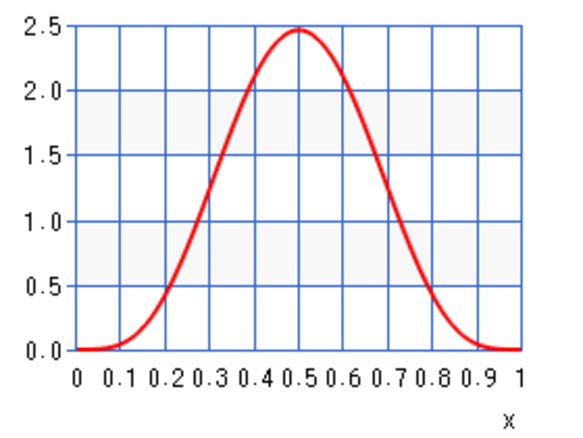
\includegraphics[width=\textwidth]{images/beta_5_5.pdf}
            \caption{$\alpha=5$, $\beta=5$}
            \label{sec:bhh:hyper_parameters:normalisation_beta_5_5}
      \end{subfigure}
      \par\bigskip
      \begin{subfigure}{0.49\textwidth}
            \centering
            \centering
            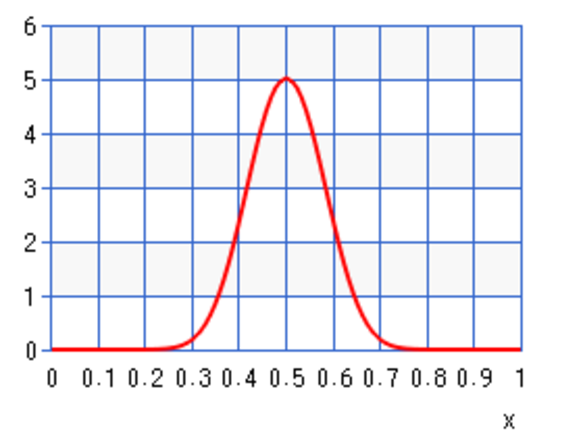
\includegraphics[width=\textwidth]{images/beta_20_20.pdf}
            \caption{$\alpha=20$, $\beta=20$}
            \label{sec:bhh:hyper_parameters:normalisation_beta_20_20}
      \end{subfigure}
      \par\bigskip
      \caption{The \index{Beta probability distribution}Beta probability distribution with varying $\alpha$ and $\beta$ values.}
      \label{sec:bhh:hyper_parameters:discounted_rewards:normalisation}
\end{figure}

\subsection{Defaults}
\label{sec:bhh:hyper_parameters:defaults}

Section \ref{sec:bhh:heuristic:proxies} provided the reader with the concept of proxied heuristic update step operations. As was mentioned in Section \ref{sec:bhh:hyper_parameters:heuristic_pool}, low-level heuristics each have their own set of hyper-parameters as well. A set of default low-level parameters must be allocated specifically for these proxies. Consider a scenario where two instances of \acs{Adam} is included in the \index{heuristic pool}heuristic pool. Each has its own set of hyper-parameters that differ from each other. In the case of \acs{Adam}, there are four hyper-parameters that include learning rate, $\eta$, $\beta_{1}$, $\beta_{2}$ and $\epsilon$. If another heuristic needs to proxy \acs{Adam}'s expected gradient mean operation, a default $\beta_{1}$ parameter must be supplied that is applied by the proxy mechanism. This is only the case when multiple instances of a heuristic is included and there is uncertainty about which instance's hyper-parameters to use for the proxied heuristic update steps. If there is only one instance of a particular heuristic, that instance's hyper-parameters are used.

\section{The \acs{BHH} Algorithm}
\label{sec:bhh:algorithm}

The high level pseudo-code implementation of the \acs{BHH} is given in Algorithm \ref{algo:bhh}.

\begin{algorithm}[htb]
      \caption{The pseudo-code for the implementation of the \acf{BHH}}
      \label{algo:bhh}
      \begin{algorithmic}
            \State step $\gets 0$

            \State select initial heuristics
            \State initialise population and entities
            \State evaluate entities' initial position
            \State update population state

            \While{stopping condition not met}
            \For{all entities in entity pool}
            \If{selected heuristic is gradient-based}
            \State get gradients
            \EndIf

            \State apply low-level heuristic and proxy operations
            \State update population state
            \State log performance metrics to performance log

            \If {step < burn-in window size}
            \State select heuristic
            \Else
            \If {step $\mathbin{\%}$ reanalysis interval = 0}
            \State apply Bayesian analysis
            \EndIf

            \If {step $\mathbin{\%}$ reselection interval = 0}
            \State select heuristic
            \EndIf

            \If {step > replay window size}
            \State prune performance log
            \EndIf
            \EndIf
            \EndFor
            \State step $\gets$ step + $1$
            \EndWhile
      \end{algorithmic}
\end{algorithm}

\section{Summary}
\label{sec:bhh:summary}

This chapter provided extensive detail on the inner workings and design of the \acs{BHH}. The \acs{BHH} was formally classified and the details around various components of the \acs{BHH}'s architecture was presented. Formal mathematical descriptions of the Bayesian selection method have been provided. The selection mechanism was presented as a probabilistic, predictive classifier. The optimisation process, by means of Bayesian analysis, has also been presented. Hyper-parameters were discussed in detail and a pseudo code implementation of the \acs{BHH} was presented.

This methodology for the empirical process is provided in the following chapter.
